\section{Results}
\begin{figure}[htbp]
\centering
\subfigure[]{
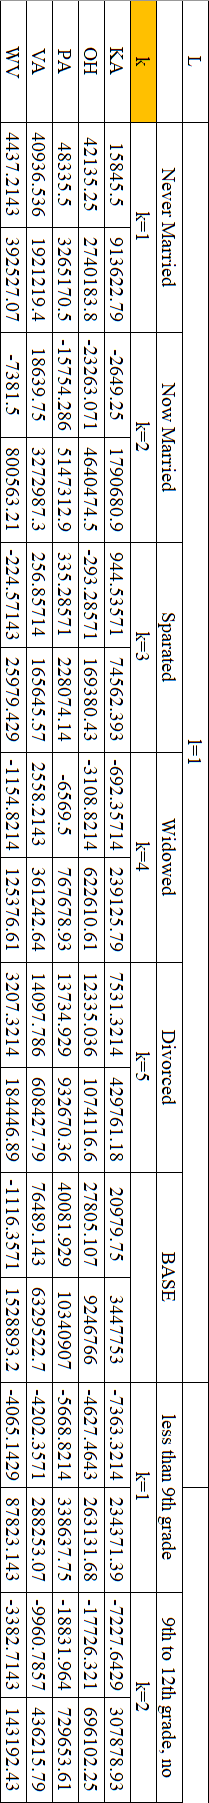
\includegraphics[scale=0.62]{regression_coefficient1.png}
}
\quad
\subfigure[]{
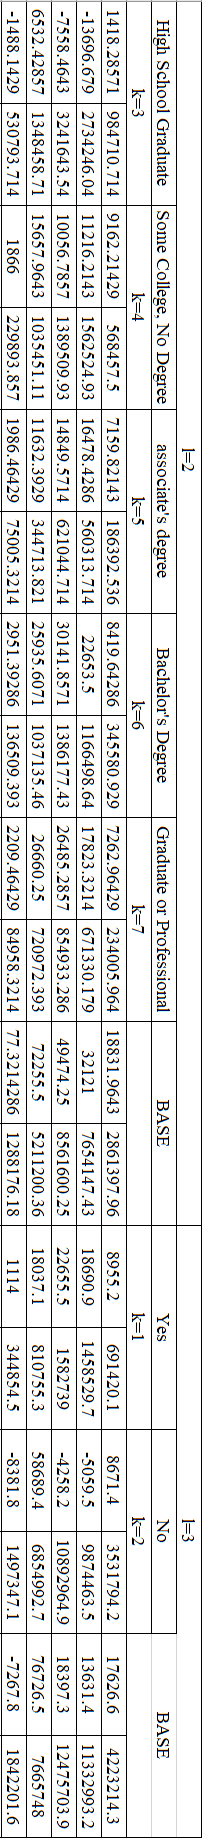
\includegraphics[scale=0.608]{regression_coefficient2.png}
}
\caption{The coefficient of linear regression for all sub-factors. The first column of each sub-factor is the linear coefficient, while the second one is the constant coefficient.}\label{regression_coefficient}
\end{figure}
